\chapter{Mérések}

Ebben a fejezetben az elvégzett mérésekről lesz szó, illetve azokból levont konklúziókról. Megnézzük, hogy a dolgozatban elkészített szoftverrendszer milyen hatékonysággal működik, milyen feltételekkel és minek milyen hatása van a QoS paraméterek elmozdulására. Kitekintünk arra, hogy egy 5G-s közeghozzáférési technológia esetén milyen változás jelenne meg a kommunikációban, elgondolkodunk rajta, hogy ez milyen előnyöket jelenthet. A méréseket az elkészített virtuális Multipass alapú K3S rendszeren végeztem, a mérési architektúra a korábbi \ref{fig:full2drone}. ábrán látható. A méréseket úgy végeztem, ahogyan a kapcsolóállomásba is implementáltam a valós idejű méréseket, annyi különbséggel, hogy nagyobb adatot átlagoltam a pontosság érdekében. \\

\noindent
Két fontos dologra vagyunk kíváncsiak:
\begin{itemize}
	\item A kapcsolóközpont viselkedése, késleltetési idő, reagálási idő
	\item A drónok számának növekedése esetén hogyan alakul a válaszidő és a sávszélesség
\end{itemize}

\section{Node váltás ideje}
A drónkapcsoló állomás hiba esetén átvált egy backup node-ra, ahol ugyanaz a munka folytatódik, amit a drón megkezdett. A kapcsolóállomásba implementált \emph{timestamp} alapú naplózórendszer segített abban, hogy pontos idők kapjak a reakcióról és a helyreállásról. Alapvetően hibát mértem, az állomás akkor is vált, ha 20\%-al jobb válaszidőt produkál egy másik worker node. A mérés menete egy drón normál üzemben működése közben:
\begin{enumerate}
	\item Hibát idézünk elő, kikapcsoljuk azt a Node-ot amelyen fut a Roscore és rögzítjük az időt (\ref{lst:close}. lista) ($t_0$)
	\item Megvárjuk amíg a kapcsolóállomás fel nem ismeri a hibát. ($t_1$)
	\item Megvárjuk amíg talál egy új Node-ot és helyreáll az üzem. ($t_2$)
\end{enumerate}

\begin{lstlisting}{caption={Node kikapcsolása}, label={lst:close}}
date +%s && multipass stop worker-1
\end{lstlisting}

$t_2-t_1$ helyreállási időre minimálisan 0.8, maximálisan 2.18, átlagosan 1.15 másodpercet mértem 10 mintavételezésből. $t_1-t_0$ észrevételi időt több periódusidővel is kipróbáltam, mindegyikkel öt-öt mérést átlagolva.
\begin{itemize}
	\item $5s$ ellenőrzési periódusidő esetén: $2.3s$
	\item $10s$ ellenőrzési periódusidő esetén: $6.1s$
	\item $15s$ ellenőrzési periódusidő esetén: $8.5s$
\end{itemize}

\noindent
Ez azt jelenti, hogy a jelentős késleltetést az ellenőrzések periódusából adódó késleltetés adja, amelynek periódusa alatt egyenesen oszlik el a várható keletkező hiba. Így annak beállítását a felhasználó mérlegelheti, hogy mennyire kritikus a drón munkája és mennyire lehet terhelni a hálózatot. Észrevétel után a kapcsolási idő már csak pár másodperc. Ha például $5s$-os hibajavítást szeretnénk, akkor $5s$-ra kell állítani az ellenőrzési periódusidőt.

\section{Terheltségi válaszidő viszonya}
Következőnek azt néztem meg, hogy a virtuális rendszerben hogyan terhelődik a klaszter az irányítandó drónok számának növekedvén. Egy drónhoz tartozik három konténer a klaszterben, abból a Roscore-ból kettő van, mindkét worker Node-on, így összesen négy konténer tartozik egy drónhoz. \\

\noindent
A válaszidőt 25 ICMP ping visszaérkezési idők átlagaként számoltam ki, úgy hogy a drón virtuális konténeréből küldtem a Roscore konténer interfészére. Az eredményen az látszik, hogy nő az üzemeltetett konténerek függvényében a válaszidő, nem drasztikusan, azonban valamilyen lineáris görbére illeszthetően (\ref{fig:meresping}. ábra).  \\

\begin{figure}
	\centering
	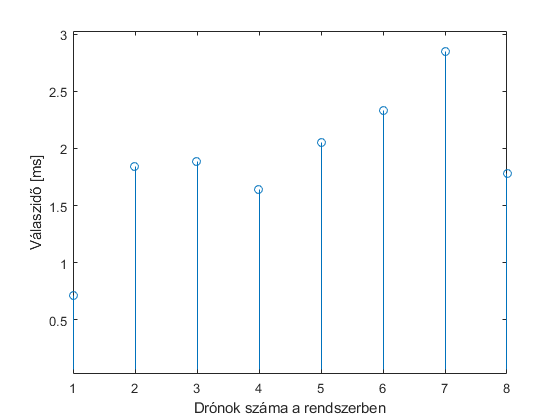
\includegraphics{figures/meres_ping.png}
	\caption{Válaszidő a drónok számának függvényében}
	\label{fig:meresping}
\end{figure}

\noindent
A sávszélességet \emph{iperf3} programmal néztem, szintén a drón konténer és a Roscore között, melyből a következő eredményt kaptam (\ref{fig:meresiperf}. ábra). A sávszélesség csökkenése is észrevehető, ugyan nincs mögötte az a linearitás, mint a válaszidő növekedésében, egy drónhoz képest megfeleződött a rendelkezésre álló kiszolgáltatott sávszélesség a klaszter felől.

\begin{figure}
	\centering
	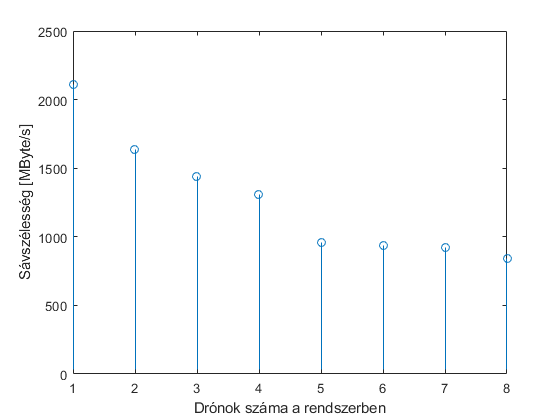
\includegraphics{figures/meres_iperf.png}
	\caption{Sávszélesség a drónok számának függvényében}
	\label{fig:meresiperf}
\end{figure}

\section{Késleltetés hozadéka 5G közeghozzáférés esetén}
A mérésekben megnéztük, hogy milyen késleltetések és sávszélességek vannak egy teljesen virtualizált rendszerben. Egy valós hálózaton és fizikai drónnal működő rendszerrel még hozzájön két érték ezekhez a késleltetésekhez és sávszélességekhez. Értelemszerűen a késleltetéshez hozzáadódik, a sávszélességnél pedig az értékek minimumára csökken. \\

\noindent
A hálózat késleltetése és a közeghozzáférési technológia késleltetése adódik hozzá a teljes válaszidőhöz. A tanszéken kipróbált Wifi-s közeghozzáférés körülbelül $300 ms$-ot növel a szimulációhoz képest. Az 5G $5-15 ms$ körüli értéket is biztosíthat, így ezzel a technológiával minimalizálni lehet a teljes késleltetést az előző pontban kiszámoltakhoz konvergálva.